\documentclass[RNAAS]{aastex62}

\newcommand{\vdag}{(v)^\dagger}
\newcommand\aastex{AAS\TeX}
\newcommand\latex{La\TeX}

\submitjournal{RNAAS}

\shorttitle{Non-Detection of Helium for WASP-12b}
\shortauthors{Kreidberg \& Oklop\v{c}i\'{c}}

\begin{document}

\title{Non-Detection of a Helium Exosphere for the Hot Jupiter WASP-12b}

\author{Laura Kreidberg}
\affiliation{Harvard-Smithsonian Center for Astrophysics, 60 Garden Street, Cambridge, MA 02138}
\affiliation{Harvard Society of Fellows, 78 Mount Auburn Street, Cambridge, MA 02138}

\author{Antonija Oklop\v{c}i\'{c}}
\affiliation{Harvard-Smithsonian Center for Astrophysics, 60 Garden Street, Cambridge, MA 02138}
A helium exosphere was recently detected around the exoplanet WASP-107b, a
low-density, warm Neptune \citep{spake18}, based on absorption features from metastable helium at $10833\,\mathrm{\AA}$ \citep[predicted
by][]{seager00,oklopcic18}. The helium feature provides a new probe of atmospheric escape that is
advantageous in several ways: (1) it is observable with near-infrared facilities
(in contrast to most other signposts of atmospheric escape that appear in the
ultraviolet) and (2) it is minimally affected by interstellar absorption,
thereby opening the door to studying atmospheric escape in a greater number of systems.

Inspired by the WASP-107b detection, we searched archival HST observations of
another evaporating exoplanet, WASP-12b, for signs of a helium exosphere.
WASP-12b is a promising 
candidate for this search because it is one of the hottest known hot
Jupiters \citep[$T_\mathrm{eq} = 2500$ K;][]{hebb09}. At this level of intense
irradiation, theory predicts a high rate of escaping atoms and molecules from
the planet's atmosphere, and indeed, transit observations in the ultraviolet
have revealed a patchy cloud of escaping material \citep{nichols15, salz16}.  

For this Note, we reanalyzed three transits of WASP-12b observed with the
Hubble Space Telescope/Wide Field Camera 3 G102 grism \citep[originally published in][]{kreidberg15b}.  In our analysis, we used the same methodology as
\cite{kreidberg15b}, except with different spectral binning to include a narrow
band ($70\,\mathrm{\AA}$, the spectrograph's native resolution) centered on the
helium feature, with two wider bands at adjacent wavelengths. 
The transmission spectrum (shown in Figure\,\ref{fig:spectrum}) is consistent with that reported in
\cite{kreidberg15b} and shows no evidence for variability between epochs.  Surprisingly, there
is no significant increase in transit depth at $10833\,\mathrm{\AA}$. The
transit depth for the helium feature is just $59 \pm 143$ ppm larger than the
weighted mean depth in the adjacent wavelength bins, in contrast to past
observations of the exosphere in the NUV, which show an increase of $\sim1\%$
relative to the optical transit depth \citep{nichols15}.

To estimate the expected absorption signal of WASP-12b at $10833\,\mathrm{\AA}$,
we used the theoretical model described in \cite{oklopcic18}.
In this 1D model, we assumed the thermosphere of the planet is composed of atomic hydrogen and helium in 9:1 number
ratio. For the thermospheric density and velocity profiles we adopted the
isothermal Parker wind model, assuming the gas temperature of $T=10^4$~K and the
total atmospheric mass loss rate of $4\times 10^{11}$~g~s$^{-1}$ \citep[based on
the results of hydrodynamic simulations of atmospheric escape in WASP-12b
by][]{salz16}. We used the solar irradiance spectrum as the input spectrum. 
We considered two density profiles of metastable helium: one calculated for the
gas at the substellar point \citep[as in][]{oklopcic18}, and the other for the
gas at the terminator, which is likely a better approximation of the average 3D
distribution of the metastable helium. We label these scenarios Model A and B,
respectively. For each profile, we predict the expected absorption signal taking into account: 1) gas within the Roche radius of the planet, where the assumptions of our 1D model are more likely to be valid, and 2) all the gas out to 20 planetary radii. 

\begin{figure*}[b!]
\begin{centering}
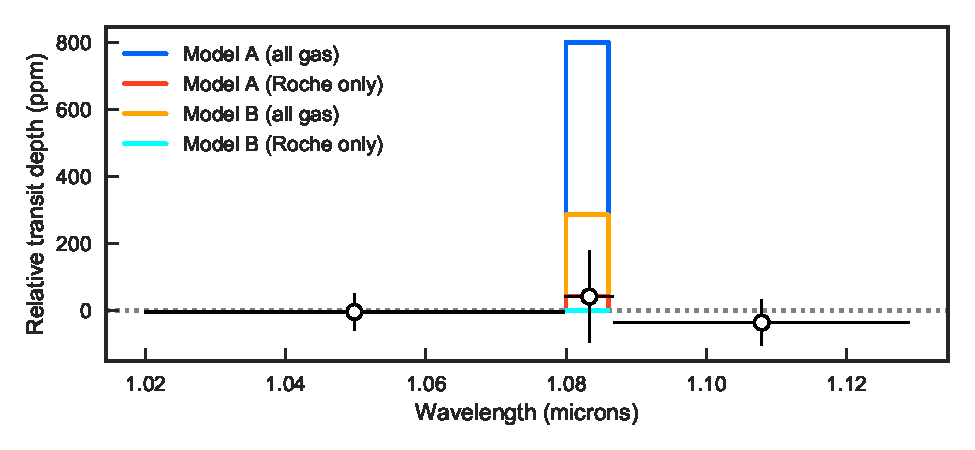
\includegraphics[width = 0.9\textwidth]{Figures/fig1.pdf}
\caption{Transmission spectrum of WASP-12b, compared to model predictions for
the strength of the $10833\mathrm{\AA}$ helium feature.}
\end{centering}
\label{fig:spectrum}
\end{figure*}

%Absorption features in this line may be smaller than in the NUV

As illustrated in Figure\,\ref{fig:spectrum}, the predicted helium feature
amplitudes are generally small and agree well with the observations. 
The least physically plausible model is ruled out (Model A with all gas, which is
inconsistent with the observed spectrum at 5.2\,$\sigma$ confidence). These
results illustrate that helium absorption may produce a much smaller feature
than atomic lines in the NUV.  In addition, there are several other factors that could weaken the helium feature even
more than what is discussed here.  One is that WASP-12 may be faint in the extreme ultraviolet (EUV). The star has
an unusually low activity level, which has been attributed to a shroud or torus of
material generated from the evaporating planet \citep{haswell17, debrecht18}. If the EUV flux
is lower than that of the Sun, the population of helium in the metastable state
will be relatively depleted, shrinking the amplitude of the helium feature.
Furthermore, if the evaporating material is distributed  in a torus around the
star, the helium absorption feature may exist at all orbital phases, not
just during the planet's transit.

In conclusion, metastable helium remains a promising probe of atmospheric
escape, but the amplitude of the signal is highly sensitive to the geometry of
the evaporating gas cloud and the input stellar spectrum.  These considerations should be taken into account in the design of future searches for helium exospheres.

 


%In conclusion, we find that WASP-12b has no evidence for a helium exosphere, in
%agreement with theoretical predictions that the helium feature amplitude should
%be small. but the
%significance of the result is dependent on the assumed geometry of the
%evaporating gas cloud as well as the input stellar spectrum.  Both of these factors should be considered in the design of future searches for helium exospheres.


\bibliographystyle{aasjournal}
\bibliography{ms.bib}

\end{document}

% End of file `sample62.tex'.
